\chapter{Logger}\label{logger}

%%%%%%%%%%  LOG4J   %%%%%%%%%%
\section{Log4j}

In prima analisi per il progetto si era pensato di utilizzare \textit{Log4j}, dato il larghissimo impiego, per il logging degli eventi da salvare poi su un file. Per poterlo utilizzare all'interno di Challenginator si sono aggiungente le dovute dipendenze, mediante \textit{Maven}, e un file \texttt{log4j2-spring.xml} dove venivano specificate le impostazioni del logger per ogni microservizio coinvolto.\\
Nel contempo però è emersa una vulnerabilità che ha scosso l'intero mondo informatico: si è scoperta la falla \textit{Log4Shell} (\texttt{CVE-2021-44228}) che permetteva ad un utente malintenzionato di controllare i messaggi di registro o i parametri dei messaggi di registro. In questa maniera era possibile eseguire codice arbitrario caricato dai server LDAP quando è abilitata la sostituzione della ricerca dei messaggi.
\begin{figure}[H]
    \centering
    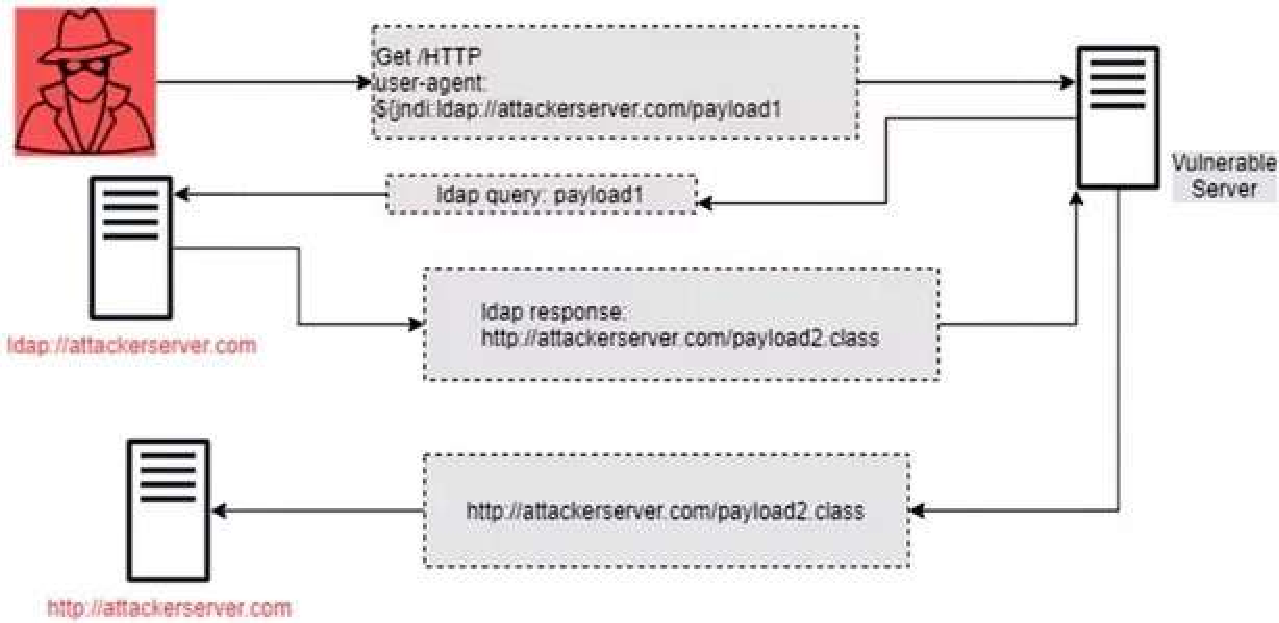
\includegraphics[width=9cm, height=4cm]{images/log4j-log4shell-bug.pdf}
    \caption{Funzionamento attacco mediante Log4Shell. Fonte: LFFL}
\end{figure}

Il CISA ha fornito una chiara rappresentazione, mediante uno schema chart, del grado di vulnerabilità del proprio sistema se si utilizza \textit{Log4j}. \cite{log4j}

\begin{figure}[H]
    \centering
    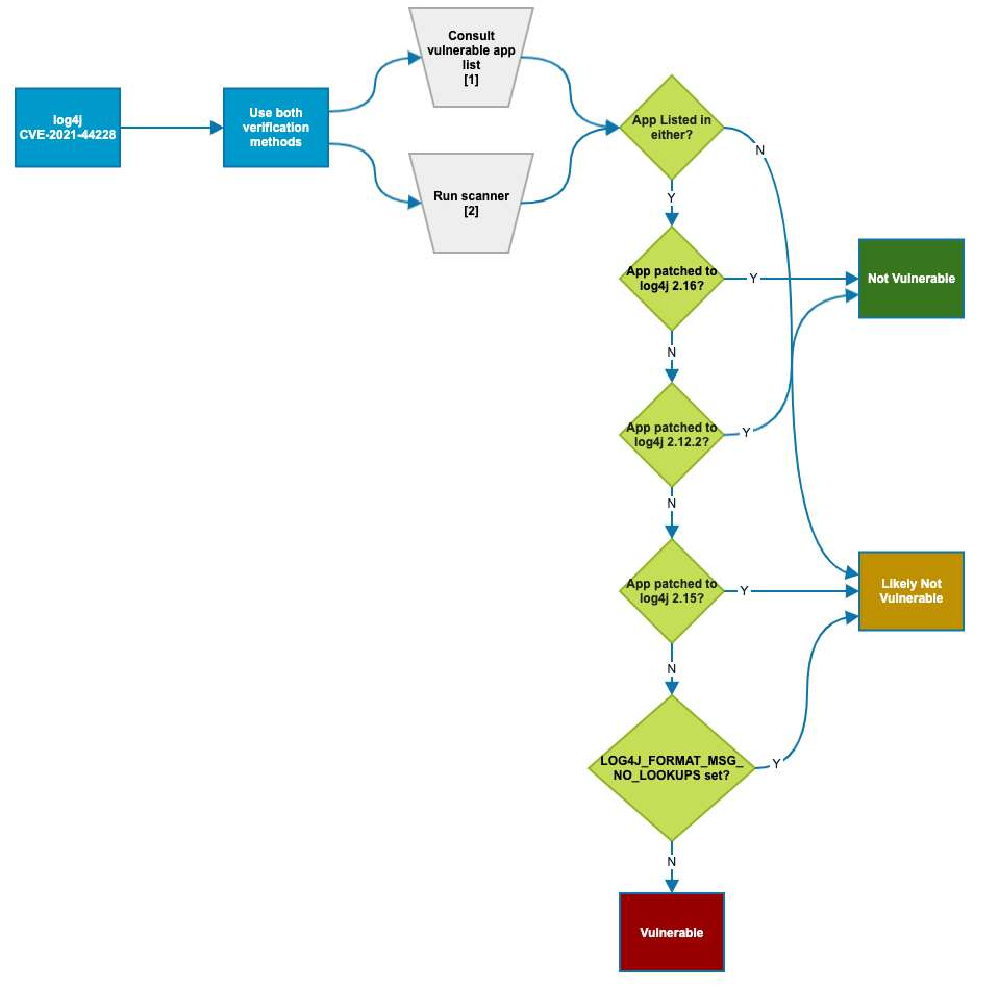
\includegraphics[width=1\textwidth]{images/log4j-bug.pdf}
    \caption{Grafico sulla vulnerabilità di prodotti che utilizzano Log4j. Fonte: CISA}
\end{figure}

Dopo questa vulnerabilità abbiamo deciso di affidarci ad un altro progetto per il logging: Logback.

%%%%%%%%%%  LOGBACK   %%%%%%%%%%
\section{Logback}

Logback \cite{logback} è uno dei più utilizzati framework per il logging nella community Java dato che, rispetto a Log4j, offre una più veloce implementazione, più opzioni di configurazione e maggiore flessibilità  nell'archiviazione di vecchi file.\\
Per inserire questo sistema di log all'interno del progetto è necessario inserire le relative dipendenze maven nel file \texttt{pom.xml}:
\begin{lstlisting}[language=XML, caption=Dipendenze Maven Logback, basicstyle=\footnotesize]
<dependency>
    <groupId>ch.qos.logback</groupId>
    <artifactId>logback-core</artifactId>
    <version>1.2.10</version>
</dependency>
<dependency>
    <groupId>ch.qos.logback</groupId>
    <artifactId>logback-classic</artifactId>
    <version>1.2.10</version>
</dependency>
<dependency>
    <groupId>org.slf4j</groupId>
    <artifactId>slf4j-api</artifactId>
    <version>1.7.32</version>
</dependency>
\end{lstlisting}

Per la configurazione è necessario creare un file di nome \texttt{logback-spring.xml} ed inserirlo nel progetto. In questo file si possono configurare gli \textit{appender}, all'interno dei quali Logback scriverà i messaggi di log; nel progetto inizialmente i log erano riportati nel terminale dell'applicazione e salvati in un file, successivamente con l'adozione di Docker venivano inviati direttamente ad una tabella del database.\\
Per poter registrare gli eventi bisogna, all'interno delle singole classi, dichiarare una variabile \texttt{Logger} ed inviare i singoli messaggi.
\begin{lstlisting}[language=Java, caption=Esempio Logger Logback, basicstyle=\footnotesize]
public class Example {
    private static final Logger logger 
      = LoggerFactory.getLogger(Example.class);

    public static void main(String[] args) {
        logger.info("Example log {}",Example.class.getSimpleName());
    }
}
\end{lstlisting}
\cite{logbackguide}.
Le funzioni da chiamare dipendono dal livello di importanza dell'informazione da trasmettere:
\begin{itemize}
    \item \texttt{.error} per il livello ERROR. Indica un errore di esecuzione o una condizione improvvisa.
    \item \texttt{.warn} per il livello WARN. Indica una condizione inaspettata o anomala di esecuzione, che però non necessariamente ha comportato un errore.
    \item \texttt{.info} per il livello INFO. Usato per segnalare gli eventi di esecuzione.
    \item \texttt{.debug} per il livello DEBUG. Usato nella fase di debug dell'applicazione.
\end{itemize}
Questa soluzione sembrava quella ottimale, ma sfortunatamente la comunicazione tra l'applicazione e il database non si instaurava e abbiamo dovuto intraprendere una nuova strada, una soluzione custom per il logging.

%%%%%%%%%%  CUSTOM LOG   %%%%%%%%%%
\section{Logger Custom}

La configurazione personalizzata è composta da  un nuovo servizio denominato \textit{logger\textunderscore service} che raccoglie tutti i messaggi di log dai vari microservizi e li invia al database ed una nuova componente in ogni microservizio atta all'invio dei messaggi di log al servizio dedicato.\\
La struttura del microservizio è riportata di seguito:
\begin{flushleft}
\dirtree{%
.1 logger\_service.
.2 controller.
.3 Controller.java.
.2 log.
.3 Log.java.
.3 LogLevel.java.
.3 LogRepository.java.
.2 messaging.
.3 LogReceiver.java.
.3 MessagingConfig.java.
.2 LogService.java.
.2 LoggerServiceApplication.java.
}
\end{flushleft}

%%%%%%%%%%  LOGGER SERVICE  %%%%%%%%%%
\subsection{Logger service}

Questo nuovo servizio è composto da principalmente tre parti:
\begin{itemize}
    \item \textit{controller}: riceve delle \textit{request} tramite URL e genera le \textit{response} corrispondenti
    \item \textit{log}: genera la classe \texttt{Log}, crea la relativa tabella nel database e si occupa delle \acrlong{jpa}
    \item \textit{messaging}: configura RabbitMQ per questo servizio, riceve le informazioni sui log dai vari microservizi e richiede il salvataggio persistente di questi ultimi 
\end{itemize}

Per la creazione del \textit{controller} si utilizzano le potenzialità del framework Spring. Mediante l'annotazione \texttt{RestController} (include le annotazioni \texttt{Controller} e \texttt{ResponseBody}) si ottiene un \textit{controller} specializzato, capace di gestire le \textit{request} mediante metodi in grado di trasformare automaticamente gli oggetti ritornati in \textit{HttpResponse}. L'annotazione \texttt{GetMapping} gestisce le chiamate GET al link specificato; tali percorsi sono esposti alla porta 8080 mediante l'\textit{API gateway}.

\begin{lstlisting}[language=Java, caption=Controller logger service, basicstyle=\footnotesize]
@RestController
public class Controller {
    @Autowired
    LogService logService;
    // restituisce tutti i log
    @GetMapping("/logs/getalllogs")
    public List<Log> getController() {
        return logService.getAll();
    }
    // controller di prova, aggiunge log fasullo
    @GetMapping("/logs/add")
    public String addLog() {
        logService.save(
            new Log(null,"now",LogLevel.WARN,"service","msg"));
        return "";
    }
}
\end{lstlisting}

L'oggetto di tipo \texttt{LogService} richiama l'omonima classe, preceduta dall'annotazione \texttt{Service} per indicare che internamente è contenuta la logica.

\begin{lstlisting}[language=Java, caption=Frammento della classe LogService, basicstyle=\footnotesize]
@Service
public class LogService {
    @Autowired
    private LogRepository logRepository;
    public void save(Log Log) {
        logRepository.save(Log);
    }
    public List<Log> getAll() {
        return logRepository.findAll();
    }
}
\end{lstlisting}

L'oggetto di tipo \texttt{LogRepository}, che richiama anch'esso l'omonima classe, è utilizzato per la comunicazione con il \gls{dbms}. Fa parte della sezione \textit{log} di questo servizio, atta alla creazione della classe \texttt{Log} e della scrittura persistente.\\
La classe \texttt{Log}, mediante l'annotazione \texttt{Entity} indica sé stessa come modello della tabella da creare nel \gls{dbms}. Le prime tre annotazioni permettono all'oggetto \texttt{id} di essere una \textit{primary key} generata automaticamente in modo incrementale, mentre \texttt{Enumerated} permette a \texttt{level} di convertire un tipo \texttt{Enum} in stringa.
\begin{lstlisting}[language=Java, caption=Frammento della classe Log, basicstyle=\footnotesize]
@Entity
public class Log {
    @Id  //PK
    @SequenceGenerator(
            name = "log_sequence",
            sequenceName = "log_sequence",
            allocationSize = 1)
    @GeneratedValue(strategy = GenerationType.SEQUENCE,
    generator = "log_sequence")
    private Long id;
    private String time;
    @Enumerated(EnumType.STRING)
    private LogLevel level;
    private String service_name;
    private String log_message;
}
\end{lstlisting}
Infine la sezione \textit{messaging} è composta da un file di configurazione per RabbitMQ in cui vengono specificati il nome della coda e dell'\textit{exchange}, e da una classe \texttt{LogReceiver} che mediante il tag \texttt{@RabbitListener} si mette in ascolto nella coda apposita per poter inviare i messaggi di log a \texttt{LogService} mediante l'annotazione \texttt{RabbitListener}
\begin{lstlisting}[language=Java, caption=Classe LogReceiver, basicstyle=\footnotesize]
@Component
public class LogReceiver {
    @Autowired
    LogService logService;
    @RabbitListener(queues = MessagingConfig.QUEUE)
    public void consumeMessageFromQueue(Log log) {
        System.out.println("\nMsg from: " + log.getService_name()
            + " with msg: \n" + log.getLog_message());
        logService.save(log);
    }
}
\end{lstlisting}

%%%%%%%%%%  COMPONENTE MICROSERVIZI %%%%%%%%%%
\subsection{Componente microservizi}

Nei vari microservizi che utilizzano questo nuovo sistema di log si sono dovute aggiungere le relative dipendenze per interfacciarsi al \acrlong{dbms}, una sezione \textit{messaging} ed un oggetto di tipo \texttt{LogService} per poter inviare i messaggi di log.
Di seguito la struttura della sezione \textit{messaging}:
\begin{flushleft}
\dirtree{%
.1 messaging.
.2 Log.java.
.2 LogLevel.java.
.2 LogService.java.
.2 MessagingConfig.java.
}
\end{flushleft}

\begin{lstlisting}[language=Java, caption=Invio dati di log, basicstyle=\footnotesize]
logService.log("Token di autenticazione creato",LogLevel.INFO);
\end{lstlisting}

La differenza tra questo servizio di log e quello precedente è che quest'ultimo si preoccupa di ricevere i dati dei log e di inviarli mediante RabbitMQ.
\begin{lstlisting}[language=Java, caption=Frammento della classe LogService - microservizi, basicstyle=\footnotesize]
@Service
public class LogService {
    @Autowired
    private RabbitTemplate template;
    @Value("${spring.application.name}")
    private String appName;
    DateTimeFormatter formatter = 
        DateTimeFormatter.ofPattern("yyyy-MM-dd HH:mm:ss");
    public Log log(String msg, LogLevel ll) {        
        Log log = new Log(null,
            LocalDateTime.now().format(formatter).toString(),
            ll,appName,msg);
        template.convertAndSend(MessagingConfig.EXCHANGE, 
            MessagingConfig.QUEUE, log);
        return log;
    }
}
\end{lstlisting}